\documentclass[titlepage]{jsarticle}
\usepackage[dvipdfmx]{graphicx}
\usepackage{amsmath}
\usepackage{amssymb}
\usepackage{amsfonts}
\usepackage{comment}
\usepackage{h31ec-exp}
\usepackage{listings}
\lstset{
    basicstyle={\ttfamily},
    identifierstyle={\small},
    commentstyle={\smallitshape},
    keywordstyle={\small\bfseries},
    ndkeywordstyle={\small},
    stringstyle={\small\ttfamily},
    frame={tb},
    breaklines=true,
    columns=[l]{fullflexible},
    numbers=left,
    xrightmargin=0zw,
    xleftmargin=3zw,
    numberstyle={\scriptsize},
    stepnumber=1,
    numbersep=1zw,
    lineskip=-0.5ex,
    keepspaces=true,
    language=c
}
\renewcommand{\lstlistingname}{リスト}
\makeatletter
\newcommand{\figcaption}[1]{\def\@captype{figure}\caption{#1}}
\newcommand{\tblcaption}[1]{\def\@captype{table}\caption{#1}}
\makeatother

\title{OPアンプの基礎・応用}
\grade{4年32番}
\author{平田 蓮}
\team{}
\date{2020年12月11日}
\expdate{2020年11月19日, 11月26日, 12月3日, 12月10日}
\coauthor{}

\begin{document}
\maketitle
\section{目的}
    本実験では, アナログ回路の素子としてよく用いられるOPアンプを用いたアナログ
    回路の中から, 増幅回路, 演算回路取り上げ, その特性を理解することを目的とする.

    まず, 基本回路として反転増幅回路の特性を理解する.
    次に, 反転増幅回路を基本とした演算増幅回路として,
    微分回路, 積分回路を取り上げる. さらに応用回路として,
    信号に含まれる特定の周波数成分を取り出すフィルタ回路を設計し,
    その周波数特性を測定する.

\section{OPアンプの基本動作}
    OPアンプについて, 詳しくは実験テキスト\cite{text}
    に載っているためここでは代表的な特徴のみ示す.

    \begin{itemize}
        \item 閉ループ利得が非常に大きい(理想的には無限大)
        \item 入力インピーダンスが非常に大きい(理想的には無限大)
        \item 出力インピーダンスが低い(理想的には$0 \ \Omega$)
    \end{itemize}

    OPアンプをアナログ回路に利用する際は負帰還回路として用いることが多い.
    今回扱う回路も全て負帰還の回路である.

\section{反転増幅回路}
    図\ref{fig:inv-amp}に反転増幅回路を示す.

    \begin{figure}[h]
        \centering
        % 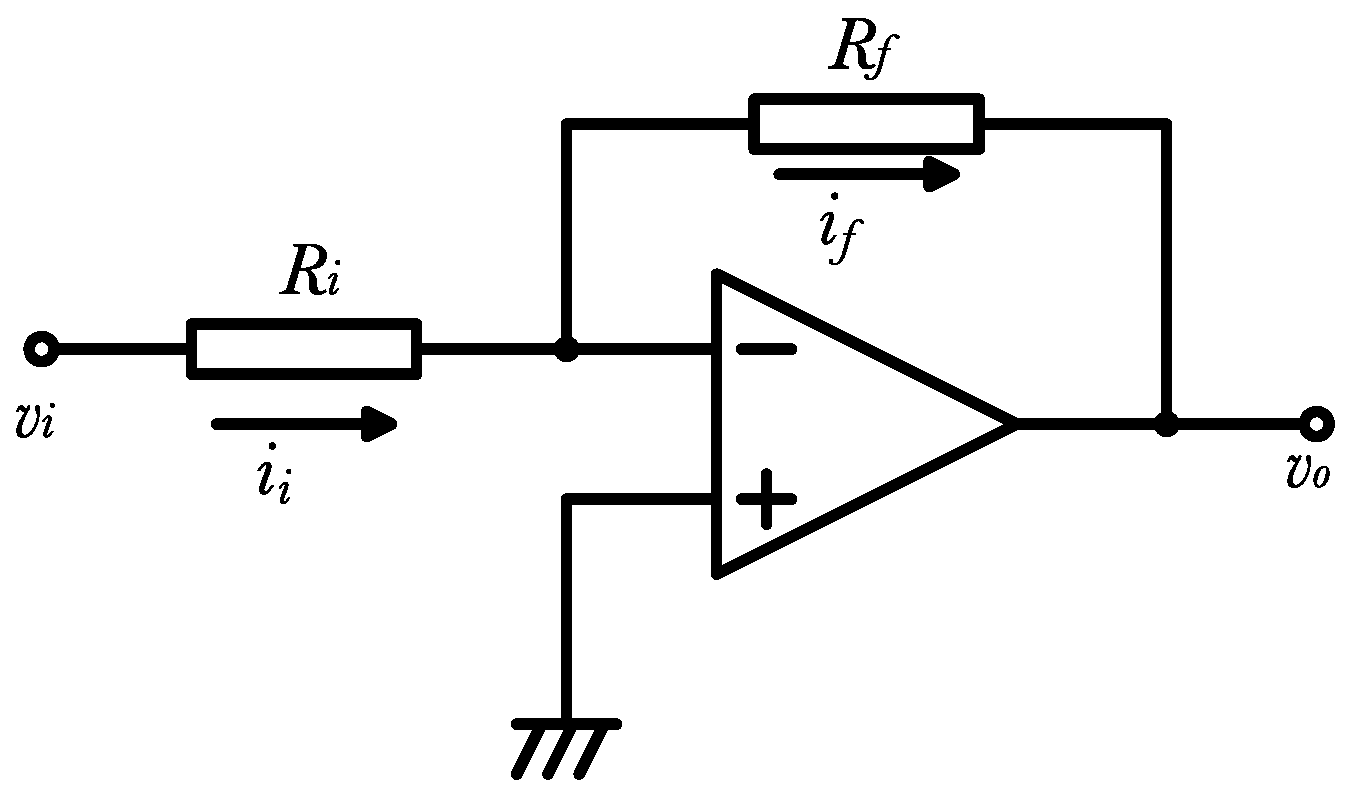
\includegraphics[0.7\hsize]{img/inv-amp.eps}
        \caption{反転増幅回路}
        \label{fig:inv-amp}
    \end{figure}

    この回路について, 閉ループ利得$A \ [倍]$, $G \ [\rm{dB}]$を求める.
    OPアンプの性質より, 二つの入力電圧を$v_s$とするとこれらは等しくなるので,
    二つの抵抗を流れる電流$i_i, i_f$について以下の式が成り立つ.

    \begin{equation*}
        i_i = \frac{v_i - v_s}{R_i} = i_f = \frac{v_s - v_o}{R_f}
    \end{equation*}

    ここで, 理想的なOPアンプでの開ループ利得を$A_0 \rightarrow \infty$とすると,
    $\displaystyle v_s = \frac{v_o}{A_0} = 0$となるので,

    \begin{equation}
        \frac{v_i}{R_i} = -\frac{v_o}{R_f} \label{equ:inv-amp}
    \end{equation}

    となる. よって, 閉ループ利得は,

    \begin{eqnarray}
        A &=& \left|\frac{v_o}{v_i}\right| = \frac{R_f}{R_i} \\
        G &=& 20 \log_{10}A
    \end{eqnarray}

    と表せる.

    \subsection{周波数特性の測定} \label{sec:ex1}
        図\ref{fig:inv-amp}の回路に振幅2V,
        周波数$f = 100 \rm{Hz} \ 〜 \ 500 \rm{kHz}$の正弦波を入力し,
        出力波形のピークピーク値$V_o \ [\rm{V}]$及び
        入力波形に対する出力波形の遅れ$t \ [\mu\rm{s}]$を測定する.

        次に,測定結果をもとに, 閉ループ利得$G \ [\rm{dB}]$及び,
        出力波形の位相の遅れ$\displaystyle\phi = 360ft \ [^\circ]$を計算する.
        
        表\ref{tab:inv-amp}に測定結果及び計算結果を示す.

        \begin{table}[h]
            \caption{各周波数に対する出力波形の振幅と, 入力に対する遅れ}
            \label{tab:inv-amp}
            \centering
            \begin{tabular}{r|rr|rr||r|rr|rr}
                $f \ [\rm{kHz}]$ & $V_o \ [\rm{V]}$ & $G \ [\rm{dB}]$ & $t \ [\mu\rm{s}]$ & $\phi \ [^\circ]$ & $f \ [\rm{kHz}]$ & $V_o \ [\rm{V]}$ & $G \ [\rm{dB}]$ & $t \ [\mu\rm{s}]$ & $\phi \ [^\circ]$ \\ \hline \hline
                0.1 & 8.0 & 6.0 & 0 & 0 & 20 & 5.4 & 2.6 & 7.5 & -54 \\
                0.2 & 8.0 & 6.0 & 0 & 0 & 30 & 3.8 & -0.4 & 6.3 & -68 \\
                0.5 & 8.0 & 6.0 & 0 & 0 & 50 & 2.3 & -4.8 & 4.5 & -81 \\
                1 & 8.0 & 6.0 & 0 & 0 & 100 & 1.1 & -11.2 & 2.5 & -90 \\
                2 & 8.0 & 6.0 & 0 & 0 & 200 & 0.5 & -18.1 & 1.4 & -101 \\
                5 & 8.0 & 6.0 & 0 & 0 & 300 & 0.3 & -21.4 & 1.1 & -119 \\
                10 & 8.0 & 6.0 & 0 & 0 & 500 & 0.2 & -26.0 & 0.8 & -135 \\
            \end{tabular}
        \end{table}

        この結果を片対数グラフにプロットしたものを図\ref{fig:inv-amp-graph1}に示す.

        \begin{figure}[h]
            \centering
            \includegraphics[width=0.8\hsize]{img/inv-amp-graph1.eps}
            \caption{反転増幅回路の周波数特性}
            \label{fig:inv-amp-graph1}
        \end{figure}

        グラフより,
        ある周波数を境に増幅率が下がりはじめ,
        位相も遅れていることがわかる.
        理論上はどんな周波数においてもOPアンプの利得は減衰しないが,
        実際の回路では高周波入力に対してOPアンプの出力が間に合わず,
        遅延が発生しているため増幅率が低下してしまうと考えられる.
        これは利得の低下とともに出力が遅延していることからもわかる.

    \subsection{課題1}
        \paragraph{
            式\ref{equ:inv-amp}の導出において,
            $A_0 \rightarrow \infty$の仮定を設けたが,
            $A_0$を有限値とした場合の式を求めよ.
        }

        \paragraph{
            式\ref{equ:inv-amp-ex}を用いて,
            $A_0$が20\%低下した場合の閉ループ利得$G$の変化を計算せよ.
            ただし, 使用するOPアンプの開ループ利得を$A_0 = 200000$とする.
        }

        \paragraph{
            十分高い周波数領域ではOPアンプの利得は-20dB/decで減衰する.
            \ref{sec:ex1}節で求めた閉ループ利得の特性線図において,
            高周波数領域の利得の現象を-20dB/decの直線で近似し,
            利得一定の直線との交点の周波数を求めよ.
        }

\section{微分回路}
    
    \subsection{基本微分回路}

        \subsubsection{入出力波形の観察}

        \subsubsection{周波数特性の測定}

    \subsection{実用微分回路}

        \subsubsection{周波数特性の測定}

    \subsection{課題2}

\section{積分回路}

    \subsection{基本積分回路}

        \subsubsection{入出力波形の観察}

        \subsubsection{周波数特性の測定}

    \subsection{実用積分回路}

        \subsection{周波数特性の測定}

    \subsection{課題3}

\section{フィルタ回路}

    \subsection{周波数特性の測定}
    
\begin{thebibliography}{99}
    \bibitem{text} OPアンプの基礎・応用, 電子制御工学実験$\cdot$ 4年後期テキスト, 2020
\end{thebibliography}
\end{document}